\documentclass[black,white]{beamer}

\usepackage{beamerthemesplit}
\usepackage{epstopdf}
\usepackage{graphicx}
\usepackage{subfigure}
\usepackage{hyperref}
\usepackage[utf8]{inputenc}
\usepackage[english]{babel}
\usepackage{listings}
\usepackage{array}
\usepackage{color}
\usepackage{colortbl}

\usefonttheme{professionalfonts}
\usecolortheme{dove}
\useoutertheme{infolines}
\useinnertheme{rectangles}

\setlength{\parindent}{0pt}
\newcommand*\sfb[1]{\textbf{#1}}
\definecolor{red2}{rgb}{.7,0,.39}
\definecolor{grey}{rgb}{0.5,0.5,0.5}
\setbeamercolor{title}{fg=white}
\setbeamercolor{frametitle}{fg=white}
\setbeamercolor{framesubtitle}{fg=white}
\setbeamercolor{normal text}{fg=white}
\setbeamercolor{itemize item}{fg=white}
\setbeamercolor{itemize subitem}{parent=itemize item}
\usebackgroundtemplate{
	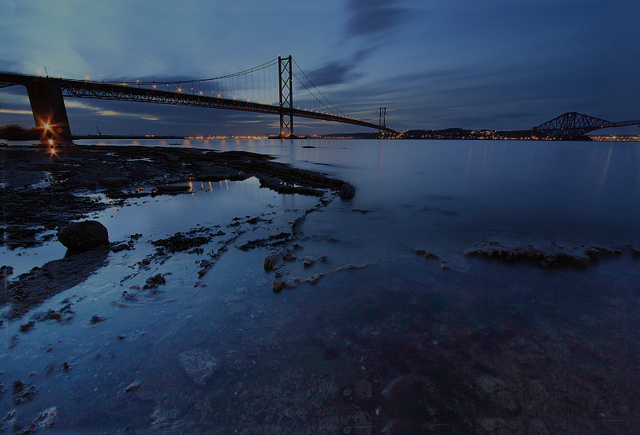
\includegraphics[width=\paperwidth,height=\paperheight]{img/bg.jpg}
}

\begin{document}

\title[netyack telephony network]{\huge{On creating a novel, future
				        global telephony network}}
\author[Daniel Borkmann] {
	\vspace*{-20pt}
	\newline
	Daniel Borkmann	\texttt{<dborkma@tik.ee.ethz.ch>}\\
	\texttt{http://gnumaniacs.org}\\\bigskip
	IET PATW 2011, Switzerland
}
\institute [ETH Zurich]{}
\date[\today]{}

\frame {
	\titlepage
}

\frame {
	\frametitle{Some notes about myself}
	\begin{itemize}
		\item 2006-2009: Technical Computer Science, B. Sc.\medskip
		\item Since 2009: Computer Science, M. Sc.\medskip
		\item Since 2011: Master thesis @ ETH Zurich\medskip
		\item Since 2009: Scholarship from the German National Merit Foundation\medskip
		\item Software development as a student worker and in my spare time\medskip
		\begin{itemize}
			\item Siemens, Max Planck Society, ipoque\medskip
			\item RoboCup, several Open Source projects
		\end{itemize}
	\end{itemize}
}

\frame {
	\frametitle{Situation among todays telecommunications}
	\begin{itemize}
		\item Oligopoly, i.e. approx 10 providers in Switzerland [1]\medskip
		\item Cost issues especially on international calls\medskip
		\item Proprietary legacy systems with security flaws [2]\medskip
		\item Privacy issues, i.e. wiretapping [3]\medskip
		\item Sparsely in focus of university research
	\end{itemize}
}

\frame {
	\frametitle{\textcolor{grey}{How others tried to challenge this:} \\\bigskip 1) Skype [5]}
	\begin{itemize}
		\item Implements VoIP, looks as an alternative on the first hand, but ...\medskip
		\item Almost everything is obfuscated, many antidebugging tricks, much ciphered code [4]\medskip
		\item Impossible to scan for trojan/backdoor/malware inclusion [4]\medskip
		\item RC4 is used for obfuscation not for privacy [4]\medskip
	\end{itemize}
}

\frame {
	\frametitle{\textcolor{grey}{How others tried to challenge this:} \\\bigskip 2) GoogleTalk/GoogleVoice}
	\begin{itemize}
		\item Also implements VoIP, proprietary like Skype\medskip
		\item No end-to-end encryption [6]\medskip
		\item Not usable by hardware phones\medskip
		\item Google seems to save your human voice for other purposes [7]\medskip
		\item Needs Adobe Flash Player (''Symantec recently highlighted Flash for having one of the worst security records in 2009.'') [8]
	\end{itemize}
}

\frame {
	\frametitle{\textcolor{grey}{How we can challenge this:} \\\bigskip Basic requirements for a new global telephony network}
	\begin{itemize}
		\item Use of a robust underlying and widespread network\medskip
		\item Compatibility with hardware phones\medskip
		\item Openness/transparency of the system\medskip
		\item (No call fees/charges)\medskip
		\item Strong cryptography between endpoints\medskip
		\item Control by users instead of companies\medskip
	\end{itemize}
}

\frame {
	\frametitle{Design of the telephony network architecture}
%
}

\frame {
	\frametitle{Design of the telephony network architecture}
%image
}

\frame {
	\frametitle{Implementation suggestions}
}

\frame {
	\frametitle{}
	\bigskip
	\bigskip
	\begin{center}
		\Large{Thanks for your attention! Questions?}\\
		\bigskip
		\bigskip
		\bigskip
		\bigskip
		\texttt{dborkma@tik.ee.ethz.ch}\\
		\medskip
		\texttt{http://gnumaniacs.org}\\
		\texttt{http://netyack.org}
	\end{center}
}

\frame {
	\frametitle{References}
	\begin{itemize}
		\item [1] http://www.telecomrating.ch/ratingaktuell.html
		\item [2] http://events.ccc.de/congress/2010/Fahrplan/events/4208.en.html
		\item [3] http://www.zdnetasia.com/beware-govts-are-tapping-your-3g-calls-62201577.htm
		\item [4] http://www.blackhat.com/presentations/bh-europe-06/bh-eu-06-biondi/bh-eu-06-biondi-up.pdf
		\item [5] http://www.nartv.org/mirror/breachingtrust.pdf
		\item [6] http://tinyurl.com/3l9pzrf
		\item [7] http://cartesianproduct.wordpress.com/2011/05/02/google-wants-your-voice/
		\item [8] http://www.apple.com/hotnews/thoughts-on-flash/
	\end{itemize}
}

\end{document}

